\documentclass{report}
\usepackage{outline}

% [outline] includes new outline environment. I. A. 1. a. (1) (a)
% use \begin{outline} \item ... \end{outline}
\usepackage{subfig}
\usepackage{graphicx}
\usepackage{times}
\usepackage{epstopdf}
\usepackage{amsmath}
\usepackage[utf8]{inputenc}
\usepackage[T1]{fontenc}
\usepackage{mathtools}
\usepackage{multirow}
\usepackage{float}
\usepackage{hyphenat}
\usepackage{color}
\usepackage{fancyhdr}
 
\pagestyle{fancy}
\fancyhf{}
\rhead{OpenFF Group}
\lhead{Bayesian Parameterization Nomenclature}
\rfoot{Page \thepage}
 

\newcommand{\cov}[1] {\mathrm{cov}\left( #1 \right)}
\newcommand{\var}[1] {\mathrm{var}\left( #1 \right)}


\title{Nomenclature for Bayesian sampling driven classical mechanics force field parameterization paper}
\author{Bryce C. Manubay}
\date{\today}
\begin{document}
{\let\newpage\relax\maketitle}
\begin{outline}
  \item{\bf Molecules}
   \begin{figure}[h!]
   \centering
  
   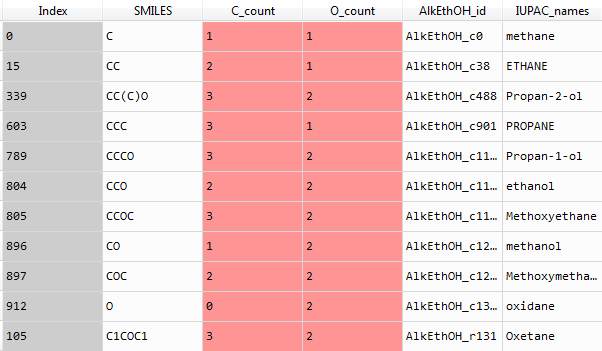
\includegraphics[width=.9\linewidth]{bayes1_mols.PNG}
   \label{fig:sub1}
   \caption{The molecules being used as the test set for this initial parameterization. Each row entry includes the SMILES string, C and O composition, ID from
            the AlkEthOH set and the IUPAC name for a given molecule.}
  
   \end{figure}
  \item{\bf Parameters **(Names given by the forcefield, will indicate differently in paper. See Nomenclature section)}
  \begin{outline}
    \item{Bond:}
      \begin{outline}
        \item{`k`: the bonded force constant $\left(\frac{kcal}{mol \cdot \AA^2} \right)$}
        \item{`length`: the equilibrium bond length $\left(\AA \right)$}
      \end{outline}
    \item{Angle:}
      \begin{outline}
        \item{`k`: the angular force constant $\left(\frac{kcal}{mol \cdot rad^2} \right)$}
        \item{`length`: the equilibrium bond angle $\left(rad \right)$}
      \end{outline}
    \item{Angle:}
      \begin{outline}
        \item{`idivfi`: barrier height divisor for torsional term i}
        \item{`ki`: force constant for torsional term i $\left(\frac{kcal}{mol} \right)$}
        \item{`phasei`: phase angle for torsional term i $\left( \deg\right)$}
        \item{`periodicityi`: periodicity of torsional term i}
      \end{outline}
  \end{outline}
  \item{\bf How many parameters?}
  \begin{outline}
    \item{Bonds (total of 5 unique SMIRKS -> 10 parameters)}
      \begin{outline}
        \item{$[\#6X4:1]-[\#6X4:2]$ (C-C)}
        \item{$[\#8:1]-[\#1:2]$ (O-H)}
        \item{$[\#6X4:1]-[\#8X2:2]$ (C-O)}
        \item{$[\#6X4:1]-[\#1:2]$ (C-H)}
        \item{$[\#6X4:1]-[\#8X2H0:2]$ (C-O where the O is bonded to another C, so ether type C-O)}
      \end{outline}
    \item{Angles (total of 3 unique SMIRKS -> 6 parameters)}
      \begin{outline}
        \item{$[\#1:1]-[\#6X4:2]-[\#1:3]$}
        \item{$[*:1]-[\#8:2]-[*:3]$}
        \item{$[*:1]~[\#6X4:2]-[*:3]$}
      \end{outline}
    \item{Torsions (torsion parameters need to be counted on a individual SMIRKS basis)}
      \begin{outline}
        \item{$[\#1:1]-[\#6X4:2]-[\#6X4:3]-[\#6X4:4]$}
          \begin{outline}
            \item{1 term}
            \item{4 total parameters}
          \end{outline}
        \item{$[\#6X4:1]-[\#6X4:2]-[\#8X2H0:3]-[\#6X4:4]$}
          \begin{outline}
            \item{2 terms}
            \item{8 total parameters}
          \end{outline}
        \item{$[*:1]-[\#6X4:2]-[\#6X4:3]-[*:4]$}
          \begin{outline}
            \item{1 term}
            \item{4 total parameters}
          \end{outline}
        \item{$[\#1:1]-[\#6X4:2]-[\#6X4:3]-[\#1:4]$}
          \begin{outline}
            \item{1 term}
            \item{4 total parameters}
          \end{outline}
        \item{$[*:1]~[*:2]~[*:3]~[*:4]$}
          \begin{outline}
            \item{1 term}
            \item{4 total parameters}
          \end{outline}
        \item{$[\#1:1]-[\#6X4:2]-[\#6X4:3]-[\#8X2:4]$}
          \begin{outline}
            \item{2 terms}
            \item{8 total parameters}
          \end{outline}
        \item{$[*:1]-[\#6X4:2]-[\#8X2:3]-[\#1:4]$}
          \begin{outline}
            \item{1 term}
            \item{4 total parameters}
          \end{outline}
        \item{$[\#6X4:1]-[\#6X4:2]-[\#8X2H1:3]-[\#1:4]$}
          \begin{outline}
            \item{2 terms}
            \item{8 total parameters}
          \end{outline}  
      \end{outline}
    \item{60 total parameters}
  \end{outline}
  \item{\bf Nomenclature:}
    \begin{outline}
    \item{Probability Terms:}
      \begin{outline}
        \item{$\hat{\Theta}$: denotes some set of parameters}
        \item{$Pr\left(\hat{\Theta}|O \right)$: posterior probability distribution; prob of some parameter set given observables}
        \item{$L\left(O|\hat{\Theta} \right)$: Likelihood function; prob of observing some observable given parameters}
        \item{$pr\left(\hat{\Theta} \right)$: prior probability; probability of parameter set based on prior knowledge}
      \end{outline}
    \item{Parameters:}
      \begin{outline}
        \item{Bonds:}
          \begin{outline}
            \item{$k_{B}$: the bonded force constant $\left(\frac{kcal}{mol \cdot \AA^2} \right)$}
            \item{$x_0$: the equilibrium bond length $\left(\AA \right)$}
          \end{outline}
        \item{Angles:}
          \begin{outline}
            \item{$k_{\theta}$: the angular force constant $\left(\frac{kcal}{mol \cdot rad^2} \right)$}
            \item{$\theta_0$: the equilibrium bond angle $\left(\deg \right)$}
          \end{outline}
        \item{Torsions:}
          \begin{outline}
            \item{$idivf_{\mathit{i}}$: barrier height divisor for torsional term i}
            \item{$k_{\mathit{i}}$: force constant for torsional term i $\left(\frac{kcal}{mol} \right)$}
            \item{$\psi_{\mathit{i}}$: phase angle for torsional term i $\left(\deg \right)$}
            \item{$\tau_{\mathit{i}}$: periodicity of torsional term i}
          \end{outline}
      \end{outline}
    \item{Observables:}
      \begin{outline}
        \item{Bonds:}
          \begin{outline}
            \item{$\mu_{B}$: mean bond length of a bond distribution $\left(\AA \right)$}
            \item{$\sigma_{B}^2$: variance in bond length of a bond distribution $\left(\AA^2 \right)$}
          \end{outline}
        \item{Angles:}
          \begin{outline}
            \item{$\mu_{\theta}$: mean bond angle of an angle distribution $\left(rad \right)$}
            \item{$\sigma_{\theta}^2$: variance in bond angle of an angle distribution $\left(rad^2 \right)$}
          \end{outline}
        \item{Torsions:}
          \begin{outline}
            \item{$A_{\mathit{i}}$: Fourier coefficient of the $i^{th}$ term}
            \item{$\psi_{\mathit{i}}$: phase angle of the $i^{th}$ term} 
            \item{$\tau_{\mathit{i}}$: periodicity of the $i^{th}$ term}
          \end{outline}
      \end{outline}
    \end{outline}   
  \end{outline} 
\end{document}
